% THIS IS AN EXAMPLE DOCUMENT FOR VLDB 2012
% based on ACM SIGPROC-SP.TEX VERSION 2.7
% Modified by  Gerald Weber <gerald@cs.auckland.ac.nz>
% Removed the requirement to include *bbl file in here. (AhmetSacan, Sep2012)
% Fixed the equation on page 3 to prevent line overflow. (AhmetSacan, Sep2012)

\documentclass{vldb}
\usepackage{graphicx}
\usepackage{balance}  % for  \balance command ON LAST PAGE  (only there!)
\usepackage{fontspec}
\setmainfont{Times}
\graphicspath{{figures/}}

\begin{document}

% ****************** TITLE ****************************************

\title{Druid: Real-time Analytical Data Store}

% possible, but not really needed or used for PVLDB:
%\subtitle{[Extended Abstract]
%\titlenote{A full version of this paper is available as\textit{Author's Guide to Preparing ACM SIG Proceedings Using \LaTeX$2_\epsilon$\ and BibTeX} at \texttt{www.acm.org/eaddress.htm}}}

% ****************** AUTHORS **************************************

% You need the command \numberofauthors to handle the 'placement
% and alignment' of the authors beneath the title.
%
% For aesthetic reasons, we recommend 'three authors at a time'
% i.e. three 'name/affiliation blocks' be placed beneath the title.
%
% NOTE: You are NOT restricted in how many 'rows' of
% "name/affiliations" may appear. We just ask that you restrict
% the number of 'columns' to three.
%
% Because of the available 'opening page real-estate'
% we ask you to refrain from putting more than six authors
% (two rows with three columns) beneath the article title.
% More than six makes the first-page appear very cluttered indeed.
%
% Use the \alignauthor commands to handle the names
% and affiliations for an 'aesthetic maximum' of six authors.
% Add names, affiliations, addresses for
% the seventh etc. author(s) as the argument for the
% \additionalauthors command.
% These 'additional authors' will be output/set for you
% without further effort on your part as the last section in
% the body of your article BEFORE References or any Appendices.

\numberofauthors{8} %  in this sample file, there are a *total*
% of EIGHT authors. SIX appear on the 'first-page' (for formatting
% reasons) and the remaining two appear in the \additionalauthors section.

\author{
% You can go ahead and credit any number of authors here,
% e.g. one 'row of three' or two rows (consisting of one row of three
% and a second row of one, two or three).
%
% The command \alignauthor (no curly braces needed) should
% precede each author name, affiliation/snail-mail address and
% e-mail address. Additionally, tag each line of
% affiliation/address with \affaddr, and tag the
% e-mail address with \email.
%
% 1st. author
\alignauthor Fangjin Yang
\email{fangjin@metamarkets.com}
\alignauthor Eric Tschetter
\email{cheddar@metamarkets.com}
\alignauthor Gian Merlino
\email{gian@metamarkets.com}
\and
\alignauthor Nelson Ray
\email{nelson@metamarkets.com}
\alignauthor Xavier L\'{e}aut\'{e}
\email{xavier@metamarkets.com}
\alignauthor Deep Ganguli
\email{deep@metamarkets.com}
}
% There's nothing stopping you putting the seventh, eighth, etc.
% author on the opening page (as the 'third row') but we ask,
% for aesthetic reasons that you place these 'additional authors'
% in the \additional authors block, viz.
\additionalauthors{Additional authors: Michael Driscoll (Metamarkets, {\texttt{mike@metamarkets.com}})}
\date{21 March 2013}
% Just remember to make sure that the TOTAL number of authors
% is the number that will appear on the first page PLUS the
% number that will appear in the \additionalauthors section.

\maketitle

\begin{abstract}
Druid is a scalable, real-time analytical data store that supports
ad-hoc queries on large-scale data sets. The system combines a
columnar data layout, a shared-nothing architecture, and an advanced
indexing structure to allow arbitrary exploration of billion-row
tables with sub-second latencies. Druid scales horizontally and is the
core engine of the Metamarkets platform. In this paper, we detail the
architecture and implementation of Druid and describe how it solves
the real-time data ingestion problem.
\end{abstract}

\section{Introduction}
In recent years, enterprises are facing ever-growing collections of
data in all forms. The scale of data has reached terabytes, even
petabytes of information per day. Companies are increasingly realizing
the importance of unlocking the insights contained within this
data. Numerous database vendors such as IBM’s Netezza \cite{singh2011introduction}, Vertica
\cite{bear2012vertica}, and EMC’s Greenplum \cite{miner2012unified} offer data warehousing solutions, and
several research papers \cite{barroso2009datacenter,
  chaudhuri1997overview, dewitt1992parallel} directly address this problem as
well. As the interactive data exploration space becomes more mature,
it is apparent that real-time ingestion and exploration of data will
unlock business-critical decisions for front office and back office
analysts.

Metamarkets realized early on that for high data volumes, existing
Relational Database Management Systems (RDBMS) and most NoSQL
architectures were not sufficient to address the performance and
use-case needs of the business intelligence space. Druid was built to
address a gap we believe exists in the current big-data ecosystem for
a real-time analytical data store. Druid is a distributed, columnar,
shared-nothing data store designed to reliably scale to petabytes of
data and thousands of cores. It is a highly available system designed
to run on commodity hardware with no downtime in the face of failures,
data imports or software updates. We have been building Druid over the
course of the last two years and it is the core engine of the
Metamarkets’ technology stack.

In many ways, Druid shares similarities with distributed databases
\cite{melnik2010dremel}, main-memory databases \cite{farber2012sap}, and widely-known distributed data
stores such as BigTable \cite{chang2008bigtable}, Dynamo \cite{decandia2007dynamo}, and Cassandra \cite{lakshman2010cassandra}. Unlike
most traditional data stores, Druid operates mainly on read-only data
and has limited functionality for writes. Druid is highly optimized
for fast aggregates over large-scale transactional data and provide a
means for deep exploration of the data. Druid is highly configurable
and allows for users to adjust levels of fault tolerance and
performance.

Druid builds on the ideas of other distributed data stores, real-time
computation engines, and search engine indexing algorithms. In this
paper, we make the following contributions to academia:
\begin{itemize}
\item We outline Druid’s real-time ingestion and query capabilities
  and explain how we can explore events within milliseconds of their
  creation
\item We describe how the architecture allows for fast and flexible
  queries and how inverted indices can be applied to quickly filter
  data
\item We present experiments benchmarking Druid’s performance
\end{itemize}
The format of the paper is as follows: Section 2 describes the Druid
data model. Section 3 presents an overview of the components of a
Druid cluster. Section 4 outlines the query API. Section 5 describes
data storage format in greater detail. Section 6 discusses Druid
robustness and failure responsiveness. Section 7 provides our
benchmarks. Section 8 lists the related work and Section 9 presents
our conclusions.

\section{Data Model}
The fundamental storage unit in Druid is the segment. Distribution and
replication in Druid are always done at a segment level. Segments
encapsulate a partition of a larger transactional data set. To better
understand how a typical row/column collection of data translates into
a Druid segment, consider the data set shown in Table~\ref{table:sample_data}.

\begin{table*}
  \centering
  \caption{Sample data}
  \label{table:sample_data}
    \begin{tabular}{| l | l | l | l | l | l | l | l | l |}
    \hline
    Timestamp & Publisher & Advertiser & Gender & Country & Impressions & Clicks & Revenue \\ \hline
    2011-01-01T01:00:00Z & bieberfever.com & google.com & Male & USA & 1800 & 25 & 15.70 \\ \hline
    2011-01-01T01:00:00Z & bieberfever.com & google.com & Male & USA & 2912 & 42 & 29.18 \\ \hline
    2011-01-01T02:00:00Z & ultratrimfast.com & google.com & Male & USA & 1953 & 17 & 17.31 \\ \hline
    2011-01-01T02:00:00Z & ultratrimfast.com & google.com & Male & USA & 3194 & 170 & 34.01 \\
    \hline
    \end{tabular}
\end{table*}

A segment is composed of multiple binary files, each representing a
column of a data set. The data set in Table~\ref{table:sample_data} consists of 8 distinct
columns, one of which is the timestamp column. Druid always requires a
timestamp column because it (currently) only operates with event-based
data. Segments always represent some interval of time and each column
file contains the specific values for that column over the time
interval. Since segments always contain data for a time range, it is
logical that Druid partitions data into smaller chunks based on the
timestamp value. In other words, segments can be thought of as blocks
of data that represent a certain granularity of time. For example, if
we wanted to shard the data in Table~\ref{table:sample_data} to an hourly granularity, the
partitioning algorithm would result in two segments, one representing
each hour of 2011-01-01. Similarly, if we sharded the data to a daily
granularity, we would create a single segment for 2011-01-01.

Partitioning the data based on granularity buckets allows users to
fine tune the degree of parallelization they want in Druid. A data set
representing a year’s worth of data may be bucketed by day, and a data
set representing only a day’s worth of day may be partitioned by
hour. Depending on the data volume, only sharding on the time
dimension may still result in segments that are too large to
manage. To create more operable partition chunks, Druid may
additionally shard data based on other factors such as dimension
cardinality. Hence, segments are uniquely identified by a data source
id describing the data, the time interval of the data, a version
indicating when the segment was created, and a shard partition number.

Data in Druid can be conceptually thought of as being either real-time
or historical. Real-time data refers to recently ingested data;
typically, in a production setting, this will be data for the current
hour. Historical data refers to any data that is older. Segments can
be similarly classified as being either real-time or historical.

Historical segments are immutable and do not support insert, delete,
or update semantics. By maintaining immutable blocks of data within
the system, we can maintain a consistent snapshot of historical
segments and provide read consistency without having to worry about
concurrent updates and deletes. If updates to a historical segment are
required, a new segment is built for the same data source and time
interval with the updated data and the version identifier is
increased. Multiple segments for the same data source and time range
may exist in the system at any time. To provide read consistency,
Druid read operations always access data in a particular time range
from the segment with the most recent version identifier for that time
range. Historical segments may be stored on local disk or in a
key-value “deep” store such as S3 \cite{decandia2007dynamo} or HDFS \cite{shvachko2010hadoop}. All historical
segments have associated metadata describing properties of the segment
such as size in bytes, compression format, and location in deep
storage.

Real-time segments are mutable and generally represent a much shorter
duration of time than historical segments. Real-time segments contain
recent data and are incrementally populated as new events are
ingested. On a periodic basis, real-time segments are converted into
historical segments. Additional details about this conversion process
are given in Section 3.3.

\section{Cluster}
A Druid cluster consists of different types of nodes, each performing
a specific function. The composition of a Druid cluster is shown in
Figure~\ref{fig:druid_cluster}.

\begin{figure}
\centering
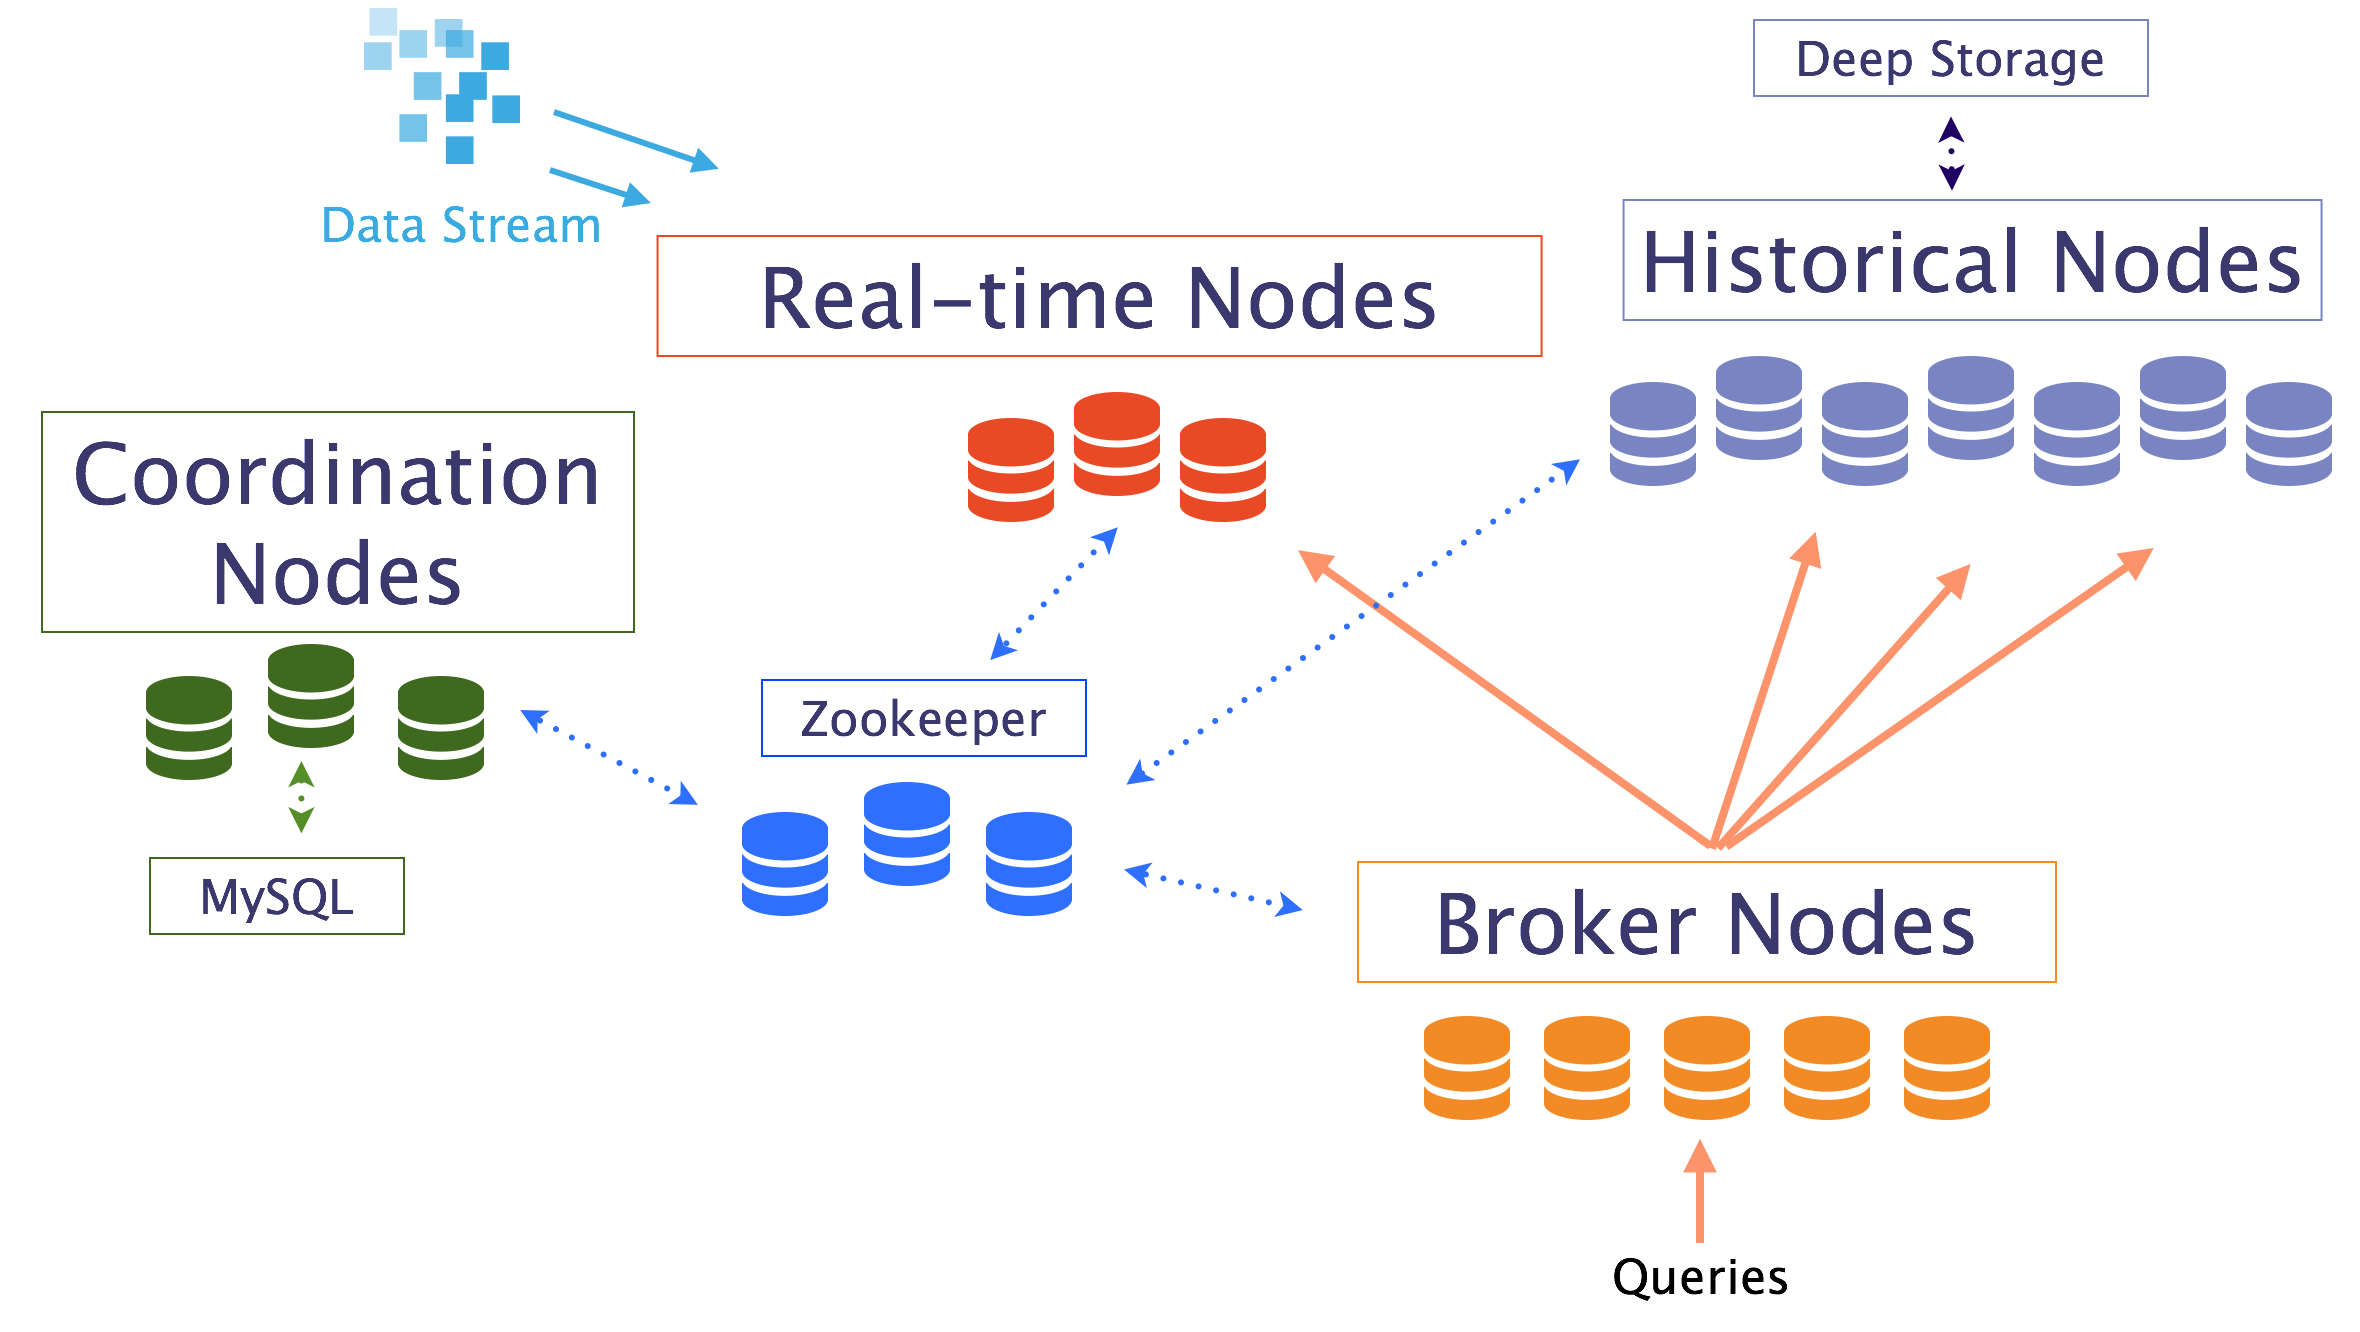
\includegraphics[width = 3in]{Druid_cluster}
\caption{An overview of a Druid cluster.}
\label{fig:druid_cluster}
\end{figure}

Recall that data in Druid is classified as either real-time or
historical. The Druid cluster is architected to reflect this
conceptual separation of data. Real-time nodes are responsible for
ingesting, storing, and responding to queries for the most recent
events. Similarly, historical compute nodes are responsible for
loading and responding to queries for historical events.

Data in Druid is stored on the compute and real-time nodes (storage
nodes). Queries to access this data will typically first hit a layer
of broker nodes. Broker nodes are responsible for finding and routing
queries down to the storage nodes that host the pertinent data. These
storage nodes compute their portion of the query response in parallel
and return their results to the brokers.

Druid also has a set of coordination nodes to manage load assignment,
distribution, and replication. Coordination nodes are not queryable
and instead focus on maintaining cluster stability.

There is minimal communication between Druid nodes and instead all
nodes connect to an Apache Zookeeper \cite{hunt2010zookeeper} cluster for
coordination. The following sections will discuss each Druid component
in greater detail.

\subsection{Apache Zookeeper}
Zookeeper is a service for coordinating processes of distributed
applications. Zookeeper provides connecting applications an
abstraction of a hierarchy of data nodes known as znodes. Each znode
is part of a hierarchical namespace, similar to file
systems. Zookeeper that has the concept of ephemeral and permanent
znodes. Permanent nodes must be created and destroyed explicitly by a
connecting application. Ephemeral znodes can be created by connecting
applications and deleted either explicitly or if the session that
created the znode is terminated (such as in the event of service
failure).

\subsection{Historical Compute Nodes}
Historical compute nodes are the main workers of a Druid cluster and
are self-contained and self-sufficient. Compute nodes load historical
segments from permanent/deep storage and expose them for
querying. There is no single point of contention between the nodes and
nodes have no knowledge of one another. Compute nodes are
operationally simple; they only know how to perform the tasks they are
assigned. To help other services discover compute nodes and the data
they hold, every compute node maintains a constant Zookeeper
connection. Compute nodes announce their online state and the segments
they serve by creating ephemeral nodes under specifically configured
Zookeeper paths. Instructions for a given compute node to load new
segments or drop existing segments are sent by creating ephemeral
znodes under a special “load queue” path associated with the compute
node.

To expose a segment for querying, a compute node must first possess a
local copy of the segment. Before a compute node downloads a segment
from deep storage, it first checks a local disk directory (cache) to
see if the segment already exists in local storage. If no cache
information about the segment is present, the compute node will
download metadata about the segment from Zookeeper. This metadata
includes information about where the segment is located in deep
storage and about how to decompress and process the segment. Once a
compute node completes processing a segment, the node announces (in
Zookeeper) that it is serving the segment. At this point, the segment
is queryable.

\subsection{Tiers}
Compute nodes can be grouped in different tiers, where all nodes in a
given tier are identically configured. Different performance and
fault-tolerance parameters can be set for each tier. The purpose of
tiered nodes is to enable higher or lower priority segments to be
distributed according to their importance. For example, it is possible
to spin up a “hot” tier of compute nodes that have a high number of
cores and a large RAM capacity. The “hot” cluster can be configured to
download more frequently accessed segments. A parallel “cold” cluster
can also be created with much less powerful backing hardware. The
“cold” cluster would only contain less frequently accessed segments.

\subsection{Real-time Nodes}
Real-time nodes encapsulate the functionality to ingest and query
real-time data streams. Data indexed via these nodes is immediately
available for querying. Real-time nodes are a consumer of data and
require a corresponding producer to provide the data
stream. Typically, for data durability purposes, a message bus such as
Kafka \cite{kreps2011kafka} sits between the producer and the real-time node as shown
in Figure~\ref{fig:data-ingestion}.

\begin{figure}
\centering
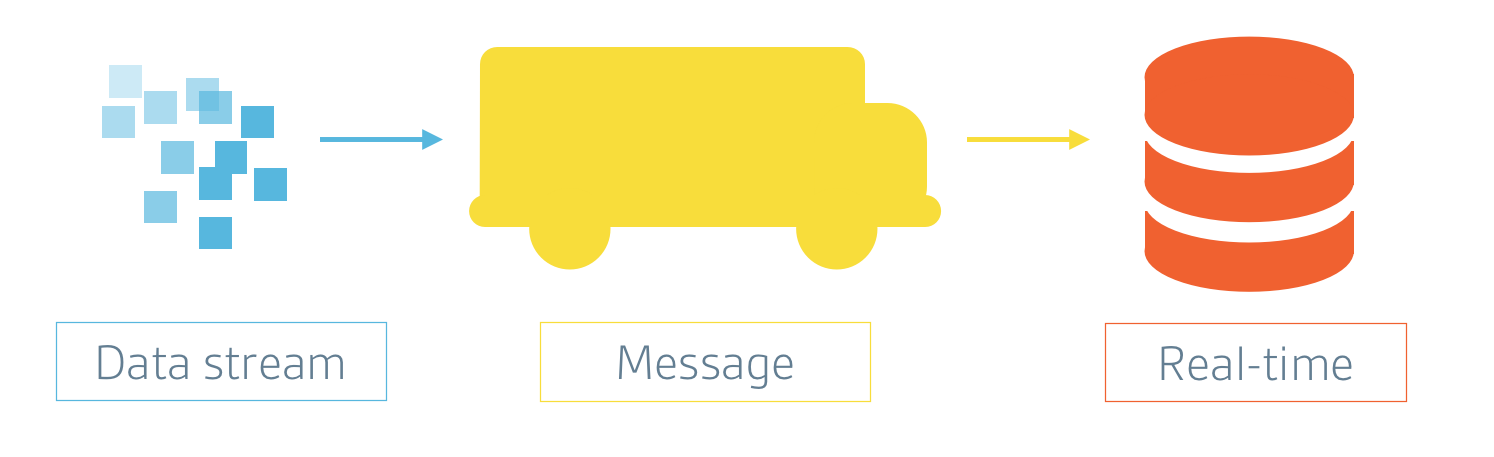
\includegraphics[width = 3in]{druid-04}
\caption{Real-time data ingestion.}
\label{fig:data-ingestion}
\end{figure}

The purpose of the message bus in Figure~\ref{fig:data-ingestion} is to act as a buffer for
incoming events. The message bus can maintain offsets indicating the
position in an event stream that a real-time node has read up to and
real-time nodes can update these offsets periodically. Real-time nodes
ingest data by reading events from the message bus.

Real-time nodes maintain an in-memory index for all incoming
events. To minimize data loss impacts, the nodes will persist their
indexes to disk either periodically or after some maximum row limit is
reached. After each persist, a real-time node updates the message bus
with the offset of the last event of the most recently persisted
index. If a real-time node fails and recovers, it can simply reload
any indexes that were persisted to disk and continue reading the
message bus from the point the last offset was committed.

Real-time nodes maintain a consolidated view of the currently updating
index and of all indexes persisted to disk. This unified view allows
all indexes to be queried. On a periodic basis, the nodes will
schedule a background task that searches for all persisted indexes of
a data source. The task merges these indexes together and builds a
historical segment. The nodes will upload the segment to deep storage
and provide a signal for the historical compute nodes to begin serving
the segment. The ingest, persist, merge, and handoff steps are fluid;
there is no data loss as a real-time node converts a real-time segment
to a historical one. Figure~\ref{fig:data-durability} illustrates the process.

\begin{figure}
\centering
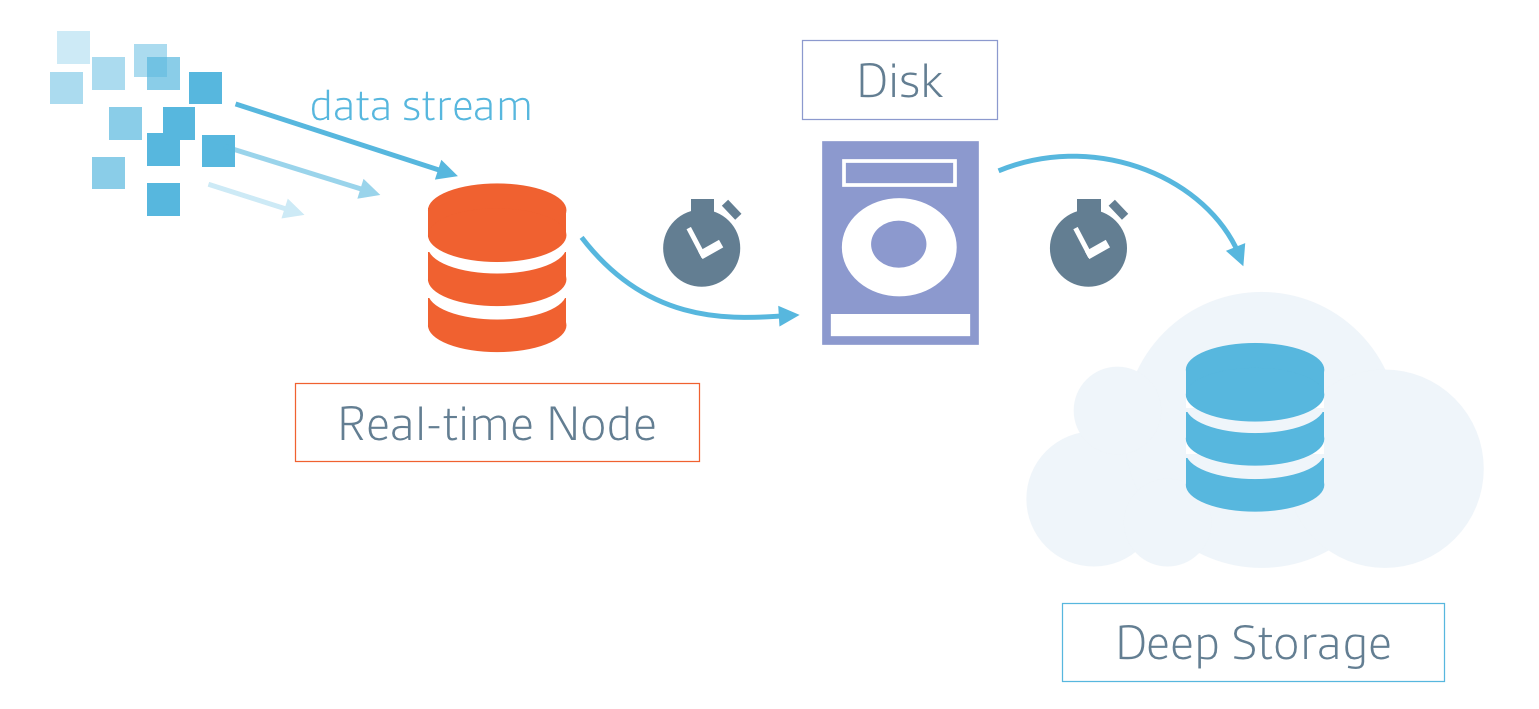
\includegraphics[width = 3in]{druid-03}
\caption{Real-time data durability}
\label{fig:data-durability}
\end{figure}

Similar to compute nodes, real-time nodes announce segments in
Zookeeper. Unlike historical segments, real-time segments may
represent a period of time that extends into the future. For example,
a real-time node may announce it is serving a segment that contains
data for the current hour. Before the end of the hour, the real-time
node continues to collect data for the hour. Every 10 minutes (the
persist period is configurable), the node will flush and persist its
in-memory index to disk. At the end of the current hour, the real-time
node prepares to serve data for the next hour by creating a new index
and announcing a new segment for the next hour. The node does not
immediately merge and build a historical segment for the previous hour
until after some window period has passed. Having a window period
allows for straggling data points to come in and minimizes the risk of
data loss. At the end of the window period, the real-time node will
merge all persisted indexes, build a historical segment for the
previous hour, and hand the segment off to historical nodes to
serve. Once the segment is queryable on the historical nodes, the
real-time node flushes all information about the segment and
unannounces it is serving the segment.

Real-time nodes are highly scalable. Multiple nodes can read the same
event stream, creating natural segment partitions across nodes. The
largest real-time Druid cluster we know of is consuming approximately
2 TB of raw data per hour.

\subsection{Broker Nodes}
Broker nodes act as query routers to other queryable nodes such as
compute and real-time nodes. Broker nodes understand the metadata
published in Zookeeper about what segments exist and on what nodes the
segments are stored. A single query will always hit a single broker
node. Broker nodes route incoming queries such that the queries hit
the right storage nodes. Broker nodes also merge partial results from
storage nodes before returning a final consolidated result to the
caller.  Additionally, brokers provide an extra level of data
durability as they maintain a cache of recent results. In the event
that multiple storage nodes fail and all copies of a segment are
somehow lost, it is still possible that segment results can still be
returned if that information exists in the cache.

\subsubsection{Timeline}
To determine the correct nodes to forward queries to, Broker nodes
first build a view of the world from information in Zookeeper. Recall
that Druid uses Zookeeper to maintain information about all compute
and real-time nodes in a cluster and the segments those nodes are
serving. For every data source in Zookeeper, the Broker node builds a
timeline of segments and the nodes that serve them. A timeline
consists of segments and represents which segments contain data for
what ranges of time. Druid may have multiple segments where the data
source and interval are the same but versions differ. The timeline
view will always surface segments that contain the most recent version
of data for a time range. When queries are received for a specific
data source and interval, the Broker node performs a lookup on the
timeline associated with the query data source for the query interval
and retrieves the segments that contain data for the query. The broker
node maps these segments to the storage nodes that serve them and
forwards the query down to the respective nodes.


\subsubsection{Caching}
Broker nodes employ a distributed cache with a LRU \cite{o1993lru, kim2001lrfu} cache
invalidation strategy. The broker cache stores per segment
results. Recall that each time a broker node receives a query, it
first maps the query to a set of segments. A subset of these segment
results may already exist in the cache and the results can be directly
pulled from the cache. For any segment results that do not exist in
the cache, the broker node will forward the query to the compute
nodes. Once the compute nodes return their results, the broker will
store those results in the cache. Real-time segments are never cached
and hence requests for real-time data will always be forwarded to
real-time nodes. Real-time data is perpetually changing and caching
the results would be unreliable.


\subsection{Coordination (Master) Nodes}
The Druid coordination or master nodes are primarily in charge of
segment management and distribution. The Druid master is responsible
for loading new segments, dropping outdated segments, managing segment
replication, and balancing segment load. Druid uses a multi-version
concurrency control swapping protocol for managing segments in order
to maintain stable views.

The Druid master runs periodically to determine the current state of
the cluster. It makes decisions by comparing the expected state of the
cluster with the actual state of the cluster at the time of the
run. As with all Druid nodes, the Druid master maintains a connection
to Zookeeper for current cluster information. The master also
maintains a connection to a MySQL database that contains additional
operational parameters and configurations. One of the key pieces of
information located in the MySQL database is a segment table that
contains a list of historical segments that should be served. This
table can be updated by any service that creates historical
segments. The MySQL database also contains a rule table that governs
how segments are created, destroyed, and replicated in the cluster.

The master does not directly communicate with a compute node when
assigning it work; instead the master creates an ephemeral node in
Zookeeper containing information about what the compute node should
do. The compute node maintains a similar connection to Zookeeper to
monitor for new work.

\subsubsection{Rules}
Historical segments are loaded and dropped from the cluster based on a
set of rules. Rules indicate how segments should be assigned to
different compute node tiers and how many replicates of a segment
should exist in each tier. Rules may also indicate when segments
should be dropped entirely from the cluster. The master loads a set of
rules from a rule table in the MySQL database. Rules may be specific
to a certain data source and/or a default set of rules can be
configured. The master will cycle through all available segments and
match each segment with the first rule that applies to it.

\subsubsection{Load Balancing}
In a typical production environment, queries often hit dozens or even
hundreds of data segments. Since each compute node has limited
resources, historical segments must be distributed among the cluster
to ensure that the cluster load is not too imbalanced. Determining
optimal load distribution requires some knowledge about query patterns
and speeds. Typically, queries cover recent data spanning contiguous
time intervals for a single data source.  On average, queries that
access smaller segments are faster.

These query patterns suggest replicating recent historical segments at
a higher rate, spreading out large segments that are close in time to
different compute nodes, and co-locating segments from different data
sources.  To optimally distribute and balance segments among the
cluster, we developed a cost-based optimization procedure that takes
into account the segment data source, recency, and size. The exact
details of the algorithm are beyond the scope of this paper.

\section{Query API}
Queries to Druid are made in the form of POST requests. All queryable
Druid nodes share the same query API. The body of the POST request is
a JSON object containing key-value pairs specifying various query
parameters. A typical query will contain the data source name, the
granularity of the result data, the time range of interest, and the
type of request.  A sample time series query is shown below:
\begin{verbatim}
{
	"queryType":"timeseries",
	"dataSource":"sample_data",
	"filter":{},
	"granularity":"day",
	"aggregations":[{"type":"count","fieldName":"row","name":"row"}],
	"intervals":"2013-01-01/2013-01-02"
}
\end{verbatim}

Certain query types will also support a filter set. A filter set is an
arbitrary Boolean expression of dimension name and value
pairs. Support for arbitrary filter sets enables flexibility and
provides the functionality to deeply explore data.

\section{Storage}
Druid is a column-oriented data store. When considering aggregates
over a large number of events, the advantages storing data as columns
rather than rows are well documented \cite{cattell2011scalable}. Column storage allows for
more efficient CPU usage as only what is needed is actually loaded and
scanned. In a row oriented data store, all columns associated with a
row must be scanned as part of an aggregation. The additional scan
time can introduce performance degradations as high as 250\% \cite{bear2012vertica}.

\subsection{Column Types}
Druid has multiple column types to represent the various column value
formats. Depending on the column type, different compression methods
are used to reduce the cost of storing a column in memory and on
disk. In the example given in Table~\ref{table:sample_data}, the
publisher, advertiser, gender, and country columns only contain
strings. String columns can be dictionary encoded. Dictionary encoding
is a common method to compress data and has been used in other data
stores such as Powerdrill \cite{hall2012processing}. In the example in
Table~\ref{table:sample_data}, we can map each publisher to an unique
integer identifier.
\begin{verbatim}
bieberfever.com -> 0
ultratrimfast.com -> 1
\end{verbatim}
This mapping allows us to represent the publisher column as an integer
array where the array indices correspond to the rows of the original
data set. For the publisher column, we can represent the unique
publishers as follows:
\begin{verbatim}
[0, 0, 1, 1]
\end{verbatim}

The resulting integer array lends itself very well to
compression. Generic compression algorithms on top of encodings are
very common in column-stores. We opted to use the LZF \cite{liblzf2013} compression
algorithm.

We can leverage similar compression algorithms for numeric
columns. For example, the clicks and revenue columns in
Table~\ref{table:sample_data} can also be expressed as individual
arrays.
\begin{verbatim}
Clicks -> [25, 42, 17, 170]
Revenue -> [15.70, 29.18, 17.31, 34.01]
\end{verbatim}
In this case we compress the raw values as opposed to their dictionary
representations.

\subsection{Filters}
To support arbitrary filter sets, Druid creates additional lookup
indices for string columns. These lookup indices are compressed and
Druid operates over the indices in their compressed form. Filters can
be expressed as Boolean equations of multiple lookup indices. Boolean
operations of indices in their compressed form is both performance and
space efficient.

Let us consider the publisher column in
Table~\ref{table:sample_data}. For each unique publisher in
Table~\ref{table:sample_data}, we can form some representation
indicating which table rows a particular publisher is seen. We can
store this information in a binary array where the array indices
represent our rows. If a particular publisher is seen in a certain
row, that array index is marked as ``1''. For example:
\begin{verbatim}
Bieberfever.com -> rows [0, 1] -> [1][1][0][0]
Ultratrimfast.com -> rows [2, 3] -> [0][0][1][1]
\end{verbatim}

Bieberfever.com is seen in rows 0 and 1. This mapping of column values
to row indices forms an inverted index \cite{tomasic1993performance}. If we want to know which
rows contain bieberfever.com OR ultratrimfast.com, we can OR together
the bieberfever.com and ultratrimfast.com arrays.
\begin{verbatim}
[0][1][0][1] OR [1][0][1][0] = [1][1][1][1]
\end{verbatim}

This approach of performing Boolean operations on large bitmap sets is
commonly used in search engines. Bitmap compression algorithms are a
well-defined area of research and often utilize run-length
encoding. Well known algorithms include Byte-aligned Bitmap Code \cite{antoshenkov1995byte},
Word-Aligned Hybrid (WAH) code \cite{wu2006optimizing}, and Partitioned Word-Aligned
Hybrid (PWAH) compression \cite{van2011memory}. Druid opted to use the CONCISE
algorithm \cite{colantonio2010concise} as it can outperform WAH by reducing the size of the
compressed bitmaps by up to 50\%.  Figure 4 illustrates the number of
bytes using CONCISE compression versus using an integer array. The
results were generated on a cc2.8xlarge system with a single thread,
2G heap, 512m young gen, and a forced GC between each run. The data
set is a single day’s worth of data collected from the Twitter garden
hose \cite{twitter2013} data stream. The data set contains 2, 272, 295 rows and 12
dimensions of varying cardinality. As an additional comparison, we
also resorted the data set rows to maximize compression.

%Figure 4. CONCISE compression versus integer array
In the unsorted case, the total CONCISE compressed size was 53, 451,
144 bytes and the total integer array size was 127, 248, 520
bytes. Overall, CONCISE compressed sets are about 42.005317\% less
than integer arrays.  In the sorted case, the total CONCISE compressed
size was 43,832,884 bytes and the total integer array size was 127,
248, 520 bytes. What is interesting to note is that after sorting,
global compression only increased minimally. The total CONCISE set
size to total integer array size is 34.448031\%. It is also
interesting to note that as the cardinality of a dimension approaches
the total number of rows in a data set, integer arrays actually
require less space than CONCISE sets.

\subsection{Storage Engine}
Druid’s persistence components allows for different storage engines to
be plugged in, similar to Dynamo \cite{decandia2007dynamo}. These storage engines may store
data in in-memory structures such as the JVM heap or in memory mapped
structures. The ability to swap storage engines allows for Druid to be
configured depending on a particular application’s specifications. An
in-memory storage engine may be operationally more expensive than a
memory-mapped storage engine but could be a better alternative if
performance is critical. At Metamarkets, we commonly use a
memory-mapped storage engine.

\section{Robustness and Fault-Tolerance}
To achieve high system availability and data durability, Druid employs
several fault recovery techniques. Druid has no single point of
failure.

\subsection{Replication}
Druid replicates historical segments on multiple hosts. The number of
replicates in each tier of the historical compute cluster is fully
configurable. Setups that require high levels of fault tolerance can
be configured to have a high number of replicates. Replicates are
assigned to compute nodes by coordination nodes using the same load
distribution algorithm discussed in section 3.5.2. Conceptually,
broker nodes do not distinguish historical segments from their
replicates. Broker nodes forward queries to the first node it finds
that contains data for the query.

Real-time segments follow a different replication model as real-time
segments are mutable. Recall that real-time nodes act as consumers of
a data stream. Multiple real-time nodes can read from the same message
bus if each maintains a unique offset, hence creating multiple copies
of a real-time segment. If a real-time node fails and recovers, it can
reload any indexes that were persisted to disk and read from the
message bus from the point it last committed an offset.

\subsection{Local Caching}
Recall that each Druid compute node maintains a local cache of
historical segments it recently served. A compute node also has a
lookup table for segments it has in its cache and stores this lookup
table on disk. When a compute node is assigned a new segment to load,
the compute node will first check its local segment cache directory to
see if the segment had been previously downloaded. If a cache entry
exists, the compute node will directly read the segment binary files
and load the segment.

The segment cache is also leveraged when a compute node is initially
started. During startup, a compute node will first read its lookup
table to determine what segments it has cached. All cached segments
are immediately loaded and served. This feature introduces minimal
overhead and allows a compute node to readily serve data as soon as it
comes online. By making data quickly available on startup and
minimizing initial startup time, compute nodes that become
inexplicably disconnected from the cluster can reconnect themselves
seamlessly. This also means that software updates can be pushed to
compute nodes without disruption to cluster operations. In practice, a
software update to a compute node can be completed before coordination
nodes even notice that the compute node has disconnected. At
Metamarkets, we update Druid through rolling restarts. Compute nodes
are updated one at a time and we experience no downtime or data loss
through the update process.

\subsection{Failure Detection}
If a compute node completely fails and becomes unavailable, the
ephemeral Zookeeper znodes it created are deleted. The master node
will notice that certain segments are insufficiently replicated or
missing altogether. Additional replicates will be created and
redistributed throughout the cluster.

We are moving towards building out infrastructure to support
programmatic creation of real-time nodes. In the near future, the
master node will also notice if real-time segments are insufficiently
replicated and automatically create additional real-time nodes as
redundant backups.

\subsection{Adding and Removing Nodes}
Starting and removing Druid nodes is a relatively simple process; all
that is required is to start and stop Java processes. There is minimal
operational overhead with adding nodes in batches. Scaling down the
cluster is usually done one node at a time with some time lapse
between shutdowns. This allows the master to have ample time to
redistribute load and create additional replicates. Shutting down
nodes in batches is generally not supported as it may destroy all
copies of a segment, which would lead to data loss.

\section{Performance Benchmarks}
To benchmark Druid performance, we created a large test cluster with
6TB of uncompressed data, representing tens of billions of fact
rows. The data set contained more than a dozen dimensions, with
cardinalities ranging double digits to tens of millions. We computed
four metrics for each row (counts, sums, and averages). The data was
sharded into chunks and each chunk was further sharded by dimension
with cardinality >> 1 million, creating thousands of shards roughly 8
million fact rows apiece.

The cluster used in the benchmark consisted of 100 historical compute
nodes, each with 16 cores, 60GB of RAM, 10 GigE Ethernet, and 1TB of
disk space. Collectively, the cluster comprised of 1600 cores, 6TB or
RAM, fast Ethernet and more than enough disk space.

On simple aggregation queries, the benchmarks of the 100 node cluster
are shown in Tables 2 - 4. SQL statements are included to describe the
purpose of the query. Please note:
\begin{itemize}
\item The timestamp range encompasses all data.
\item 15-core is a 16-core machine with 60GB RAM and 1TB of local
  disk.  The machine was configured to only use 15 threads for
  processing queries.
\item 4-core is a 4-core machine with 32GB RAM and 1TB of local disk.
\item ``in-memory'' means that the machine was configured to load all
  data up into the Java heap and have it available for querying
\item ``mmap'' means that the machine was configured to mmap the data
  instead of load it into the Java heap
\end{itemize}

\begin{figure}
\centering
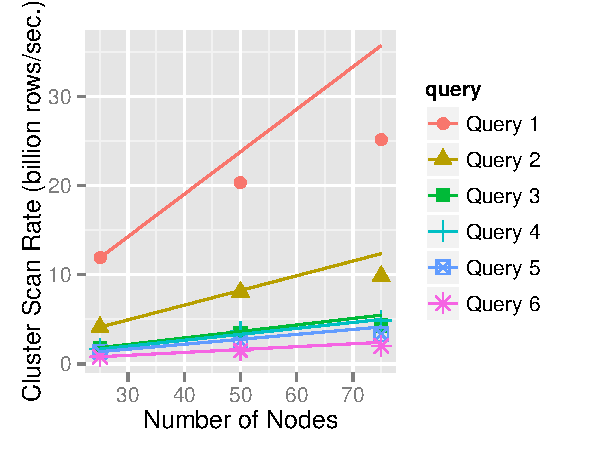
\includegraphics[width = 3in]{cluster_scan_rate}
\caption{Druid cluster scan rate.}
\label{fig:cluster_scan_rate}
\end{figure}

\begin{table*}
  \centering
  \caption{Druid Queries}
  \label{table:sql_queries}
    \begin{tabular}{| l | l |}
    \hline
    Query \# & Query \\ \hline
    1 & Select count(*) from \_table\_ where timestamp $\geq$ ? and timestamp $<$ ?; \\ \hline
    2 & Select count(*), sum(metric1) from \_table\_ where timestamp $\geq$ ? and timestamp $<$ ?; \\ \hline
    3 & Select count(*), sum(metric1), sum(metric2), sum(metric3), sum(metric4) where timestamp $\geq$ ? and timestamp $<$ ?; \\ \hline
    4 & Select high\_card\_dimension, count(*) AS cnt from \_table\_ where timestamp $\geq$ ? and timestamp $<$ ? group by high\_card\_dimension order by cnt limit 100; \\ \hline
    5 & Select high\_card\_dimension, count(*), sum(metric1) AS cnt from \_table\_ where timestamp $\geq$ ? and timestamp $<$ ? group by high\_card\_dimension order by cnt limit 100; \\ \hline
    6 & Select high\_card\_dimension, count(*), sum(metric1), sum(metric2), sum(metric3), sum(metric4) AS cnt from \_table\_ where timestamp $\geq$ ? and timestamp $<$ ? group by high\_card\_dimension order by cnt limit 100; \\
    \hline
    \end{tabular}
\end{table*}

% \begin{enumerate}
% \item \texttt{Select high\_card\_dimension, count(*), sum(metric1), sum(metric2), sum(metric3), sum(metric4) AS cnt from \_table\_ where timestamp $\geq$ ? and timestamp $<$ ? group by high\_card\_dimension order by cnt limit 100;}
% \end{enumerate}

The first query listed in Table 2 is just a count and we see the best
performance of our system with it, achieving scan rates of 33M
rows/second/core.  At first glance it looks like fewer nodes might
actually be outperforming more nodes in the rows/sec/core metric, but
that's just because 100 nodes is over provisioned for the data set.
Druid's concurrency model is based on shards, one thread will scan one
shard.  If a node has 15 cores, for example, and handles a query that
requires scanning 16 shards, if we assume each shard takes 1 second to
process the total time to finish the query will be 2 seconds (1 second
for the first 15 shards and 1 second for the 16th shard), decreasing
the global scan rate because there are actually a number of cores that
are idle.

When we include more aggregations we see performance degrade.  This is
because of the column-oriented storage format Druid employs.  For the
count(*) queries, it only has to check the timestamp column to satisfy
the where clause.  As we add metrics, it has to also load those metric
values and scan over them, increasing the amount of memory scanned.
Table 5-7 shows the results for top 100 queries on our high
cardinality dimension.

In Tables 5-7, we see the superior performance of the in-memory
representation when doing top lists versus when doing simple
time-based aggregations.  This is an implementation detail, but it's
largely because of the differences in accessing simple in-memory
pointers, versus scanning and seeking through a flattened data
structure (even though it is already largely paged into memory).

\section{Related Work}
Cattell \cite{cattell2011scalable} maintains a great summary about existing Scalable SQL and
NoSQL data stores. In the landscape of distributed data stores, Druid
feature-wise sits somewhere between Google’s Dremel \cite{melnik2010dremel} and Powerdrill
\cite{hall2012processing}. Druid has most of the features implemented in Dremel (Dremel
handles arbitrary nested data structures while Druid only allows for a
single level of array-based nesting) and many of the interesting
compression algorithms mentioned in Powerdrill.

Although Druid builds on many of the same principles as other
distributed column-oriented data stores \cite{fink2012distributed}, most existing data
stores are designed to be key-value stores \cite{lerner2010redis}, or
document/extensible record stores \cite{stonebraker2005c}. Such data stores are great
solutions for traditional data warehouse needs and general
back-office/reporting usage. Typically, analysts will query these data
stores and build reports from the results. In-memory databases such as
SAP’s HANA \cite{farber2012sap} and VoltDB \cite{voltdb2010voltdb} are examples of other data stores that
are highly suited for traditional data warehousing needs. Druid is a
front-office system designed such that user-facing dashboards that be
built on top of it. Similar to \cite{paraccel2013}, Druid has analytical features
built in. The main features Druid offers over traditional data
warehousing solutions are real-time data ingestion, interactive
queries and interactive query latencies. In terms of real-time
ingestion and processing of data, Trident/Storm \cite{marz2013storm} and Streaming
Spark \cite{zaharia2012discretized} are other popular real-time computation systems, although
they lack the data storage capabilities of Druid. Spark/Shark \cite{engle2012shark} are
also doing similar work in the area of fast data analysis on large
scale data sets. Cloudera Impala \cite{cloudera2013} is another system focused on
optimizing querying performance, but more so in Hadoop environments.

Druid leverages a unique combination of algorithms in its
architecture. Although we believe no other data store has the same set
of functionality as Druid, some of Druid’s features such as using
inverted indices to perform faster filters also exist in other data
stores \cite{macnicol2004sybase}.

\section{Conclusions}
In this paper, we presented Druid, a distributed, column-oriented,
real-time analytical data store. Druid is a highly customizable
solution that is optimized for fast query latencies. Druid ingests
data in real-time and is fault-tolerant. We discussed the performance
of Druid on billion row data sets. We discussed key Druid architecture
aspects such as the storage format, query language and general
execution. In the future, we plan to cover more in depth the different
algorithms we’ve developed for Druid and how other systems may plug
into Druid to achieve powerful use cases.

\section{Acknowledgements}
Druid could not have been built without the help of many great
engineers at Metamarkets and in the community. We want to thank Steve
Harris, Jaypal Sethi, Danny Yuan, Jae Hyeon Bae, Paul Baclace, Dave
Nielsen, Katherine Chu, and Dhruv Parthasarathy for their
contributions to Druid.

% The following two commands are all you need in the
% initial runs of your .tex file to
% produce the bibliography for the citations in your paper.
\bibliographystyle{abbrv}
\bibliography{druid}  % druid.bib is the name of the Bibliography in this case
% You must have a proper ".bib" file
%  and remember to run:
% latex bibtex latex latex
% to resolve all references

%Generated by bibtex from your ~.bib file.  Run latex,
%then bibtex, then latex twice (to resolve references).

%APPENDIX is optional.
% ****************** APPENDIX **************************************
% Example of an appendix; typically would start on a new page
%pagebreak

\end{document}